\section{Application of Principal Component Analysis on Acoustic Signals via R}


With the processed data, original and spectrum, we can proceed with the application of PCA. The actual application of PCA via R is simply performed by the built-in function \emph{prcomp}() \cite{Chazal}.


\subsection{PCA on original dataframe}


By inserting original data frame as the input variable on the function \emph{prcomp}(), we generate a PCA processed data and store it in the variable \emph{my-pca}. 

The resulting object \emph{my-pca} is a large prcomp-type data with 5 elements: \emph{sdev, rotation, center, scale, x}. The \emph{sdev} holds the standard deviation for each 219 principal components, and the other four elements holds 219 data of the relevant information for each 219 principal components. Therefore, \emph{my-pca} stores 219 elements, each representing a principal component, which are each 219 length, thus comprising a 219 x 219 dataframe.

The 219 principal components processed in \emph{my-pca} are ordered from highest variance to the lowest, meaning the first few principal components are the most important data to look into. We would select the first three principal components, naming each of them \emph{PC1, PC2, PC3}, and construct three different biplots by putting x and y axis with the combinations of these three principal components.

\begin{figure}[H]
    \centering
    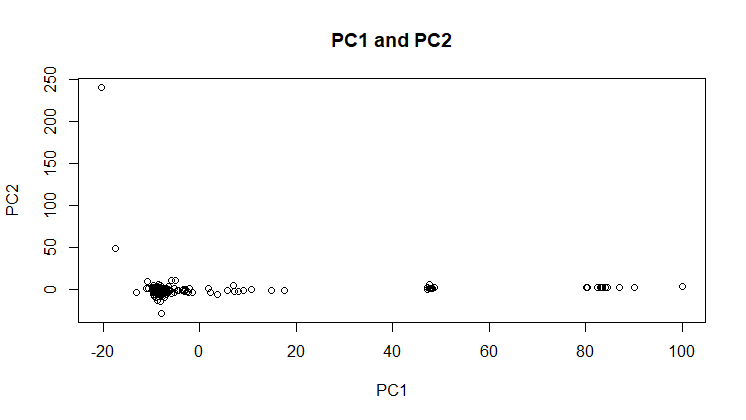
\includegraphics[width=12cm]{images/PCA/PC1 and PC2.png}   
    \caption{Biplot of PC1 and PC2}
    \label{fig:PCA12biplot} 
\end{figure}

\begin{figure}[H]
    \centering
    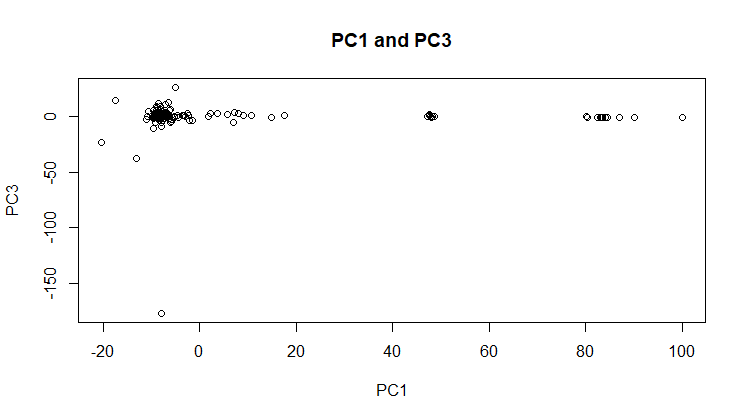
\includegraphics[width=12cm]{images/PCA/PC1 and PC3.png}
    \caption{Biplot of PC1 and PC3}
    \label{fig:PCA13biplot} 
\end{figure}

\begin{figure}[H]
    \centering
    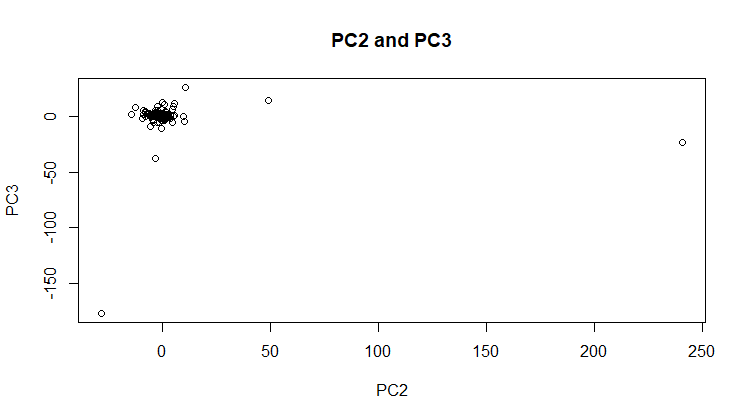
\includegraphics[width=12cm]{images/PCA/PC2 and PC3.png}
    \caption{Biplot of PC2 and PC3}
    \label{fig:PCA23biplotd} 
\end{figure}

We can analyze the nature of each principal components by observing the points on these biplots \cite{PCAbiplot}. The corresponding score of each points along the x and y axis is proportionate to the strength regarding the principal component of the axis. 

For instance, if we closely examine figure 7 and figure 8 we notice that there are several points heading to the far right along the x-axis, which is PC1. This tells that these points have strong scores on the PC1 component. 

The cluster of the points also describes the relative character and the general structure of the principal components. If we observe figure 1, we can confirm that there exists a central cluster near value -10 for PC1 and value 0 for PC2. We can also confirm that there lies a single point on the far up-left corner. This single point can be interpreted as an outlier for the PC2 component, as the 219 points for PC2 are mostly distributed near value 0 and forms a strong cluster group around the are.

The same attribute can be confirmed from PC3 component as well by observing figure 2. Most of the points are distributed near the value of 0 and forms a strong cluster group near the are, and there lies a single outlier on the bottom-left corner of the plot. By observing figure 9, where the cluster group is most heavily centered near the value 0 for both PC2 and PC3, we can observe that PC1 forms higher variance compared to PC2 and PC3

Now we should compute the variance in order to calculate the number of principal components to use and to neglect in order to reduce the dimension of the data. We can square the standard deviation given from the element \emph{sdev} from \emph{my-pca} to calculate the variance of each 217 principal components.

Then we calculate the proportion of variance of each principal components by dividing each variance with the total sum of 219 variances. We can now plot a scree plot with x-axis being the principal components and y-axis being the proportion of variance of the principal components.

\begin{figure}[H]
    \centering
    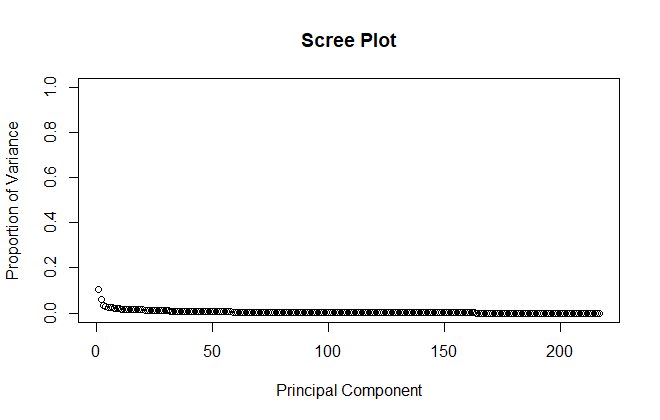
\includegraphics[width=12cm]{images/PCA/Scree Plot.png}
    \caption{Scree Plot}
    \label{fig:screeplot} 
\end{figure}

We can also construct a cumulative scree plot, which has y-axis as the cumulative proportion of variance instead.

\begin{figure}[H]
    \centering
    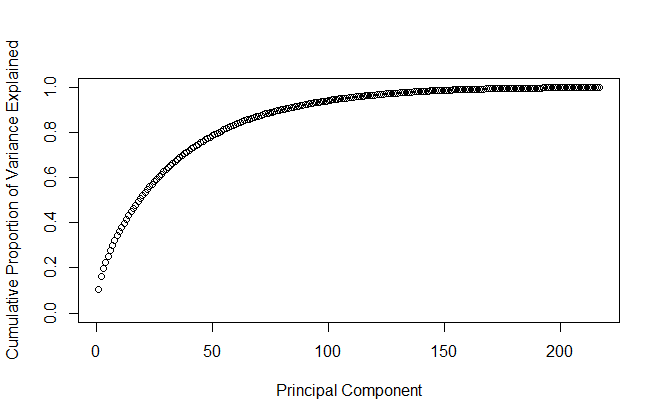
\includegraphics[width=12cm]{images/PCA/Cumulative Scree Plot.png}
    \caption{Cumulative Scree Plot}
    \label{fig:cumscreeplot} 
\end{figure}

We can notice from the plot that the first three principal components contributes to roughly 20 percent of the total variance and the first 12 principal components contributes to roughly 40 percent of the total variance.

We can now compute the number of principal components (chosen by the given order since it is already arranged by variance) to use and to neglect, depending on the percentage of the variance. In order to take account of 80 percent of the variance we get a calculated result of 53 (roughly 75.5 percent reduction in dimension). In order for 90 percent and 95 percent we get a calculated result of 79 (roughly 64 percent reduction in dimension) and 105 (roughly 52 percent reduction in dimension) each. 

In conclusion the overall result of the principal component analysis applied on interpolated 219 acoustic signal data resulted on generating 219 principal components. By calculating the proportion of variance, we concluded with a calculation that roughly 75.5, 64, and 52 percent of dimension out of 219 dimensions can be reduced in order to consider 80, 90, 95 percent of the total variance. 


\newpage
\subsection{PCA on Spectrum}


We can apply PCA on the spectrum dataframe \emph{finalSpec} through similar process as we did in the above section. The key difference between the two dataframes is in the length of each variables: the number of columns. While the original interpolated dataframe has 5,000 columns, the spectrum dataframe has 19,456 columns. The difference, however, does not heavily affect in the general results as the dimension of the principal components remains the same since as each of the 219 rows of two dataframes relates to the same acoustic signals.

We insert \emph{finalSpec} into function \emph{prcomp}() and store the result in object \emph{my-pca}. 

The resulting data \emph{my-pca} consists with 5 elements: \emph{sdev, rotation, center, scale, x}. The \emph{sdev} holds the standard deviation for each 219 principal components of the spectrum dataframe, and the other four elements holds 219 data of the relevant information for each 219 principal components. 

Now we construct the biplots of the firs three principal components.

\begin{figure}[H]
    \centering
    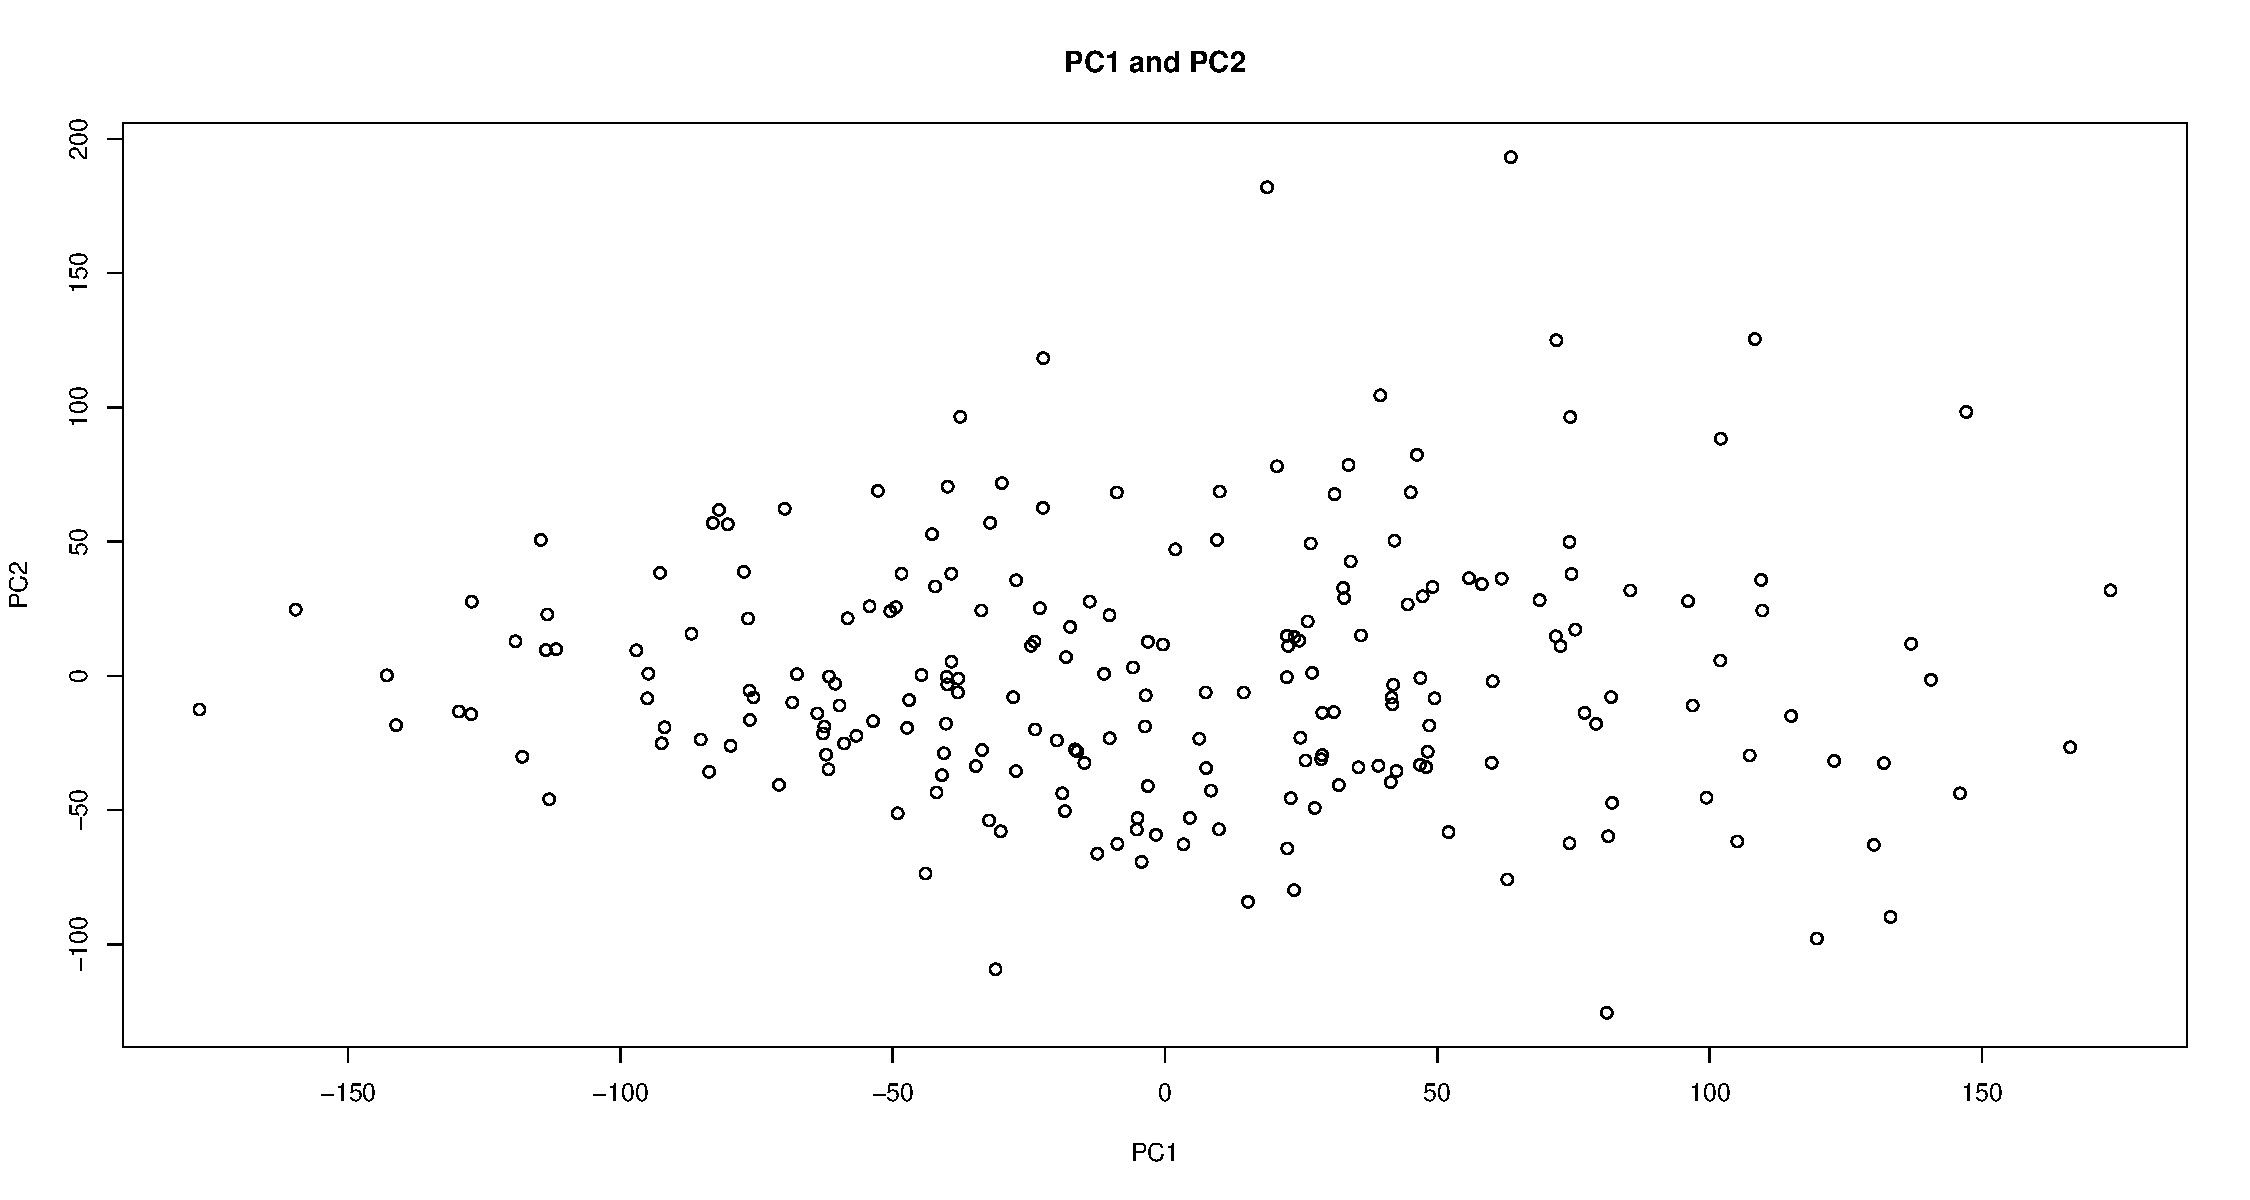
\includegraphics[width=12cm]{images/PCA (Spec)/PC1 and PC2.pdf}  
    \caption{Biplot of Spectrum's PC1 and PC2}
    \label{fig:PCASpec12biplot} 
\end{figure}

\begin{figure}[H]
    \centering
    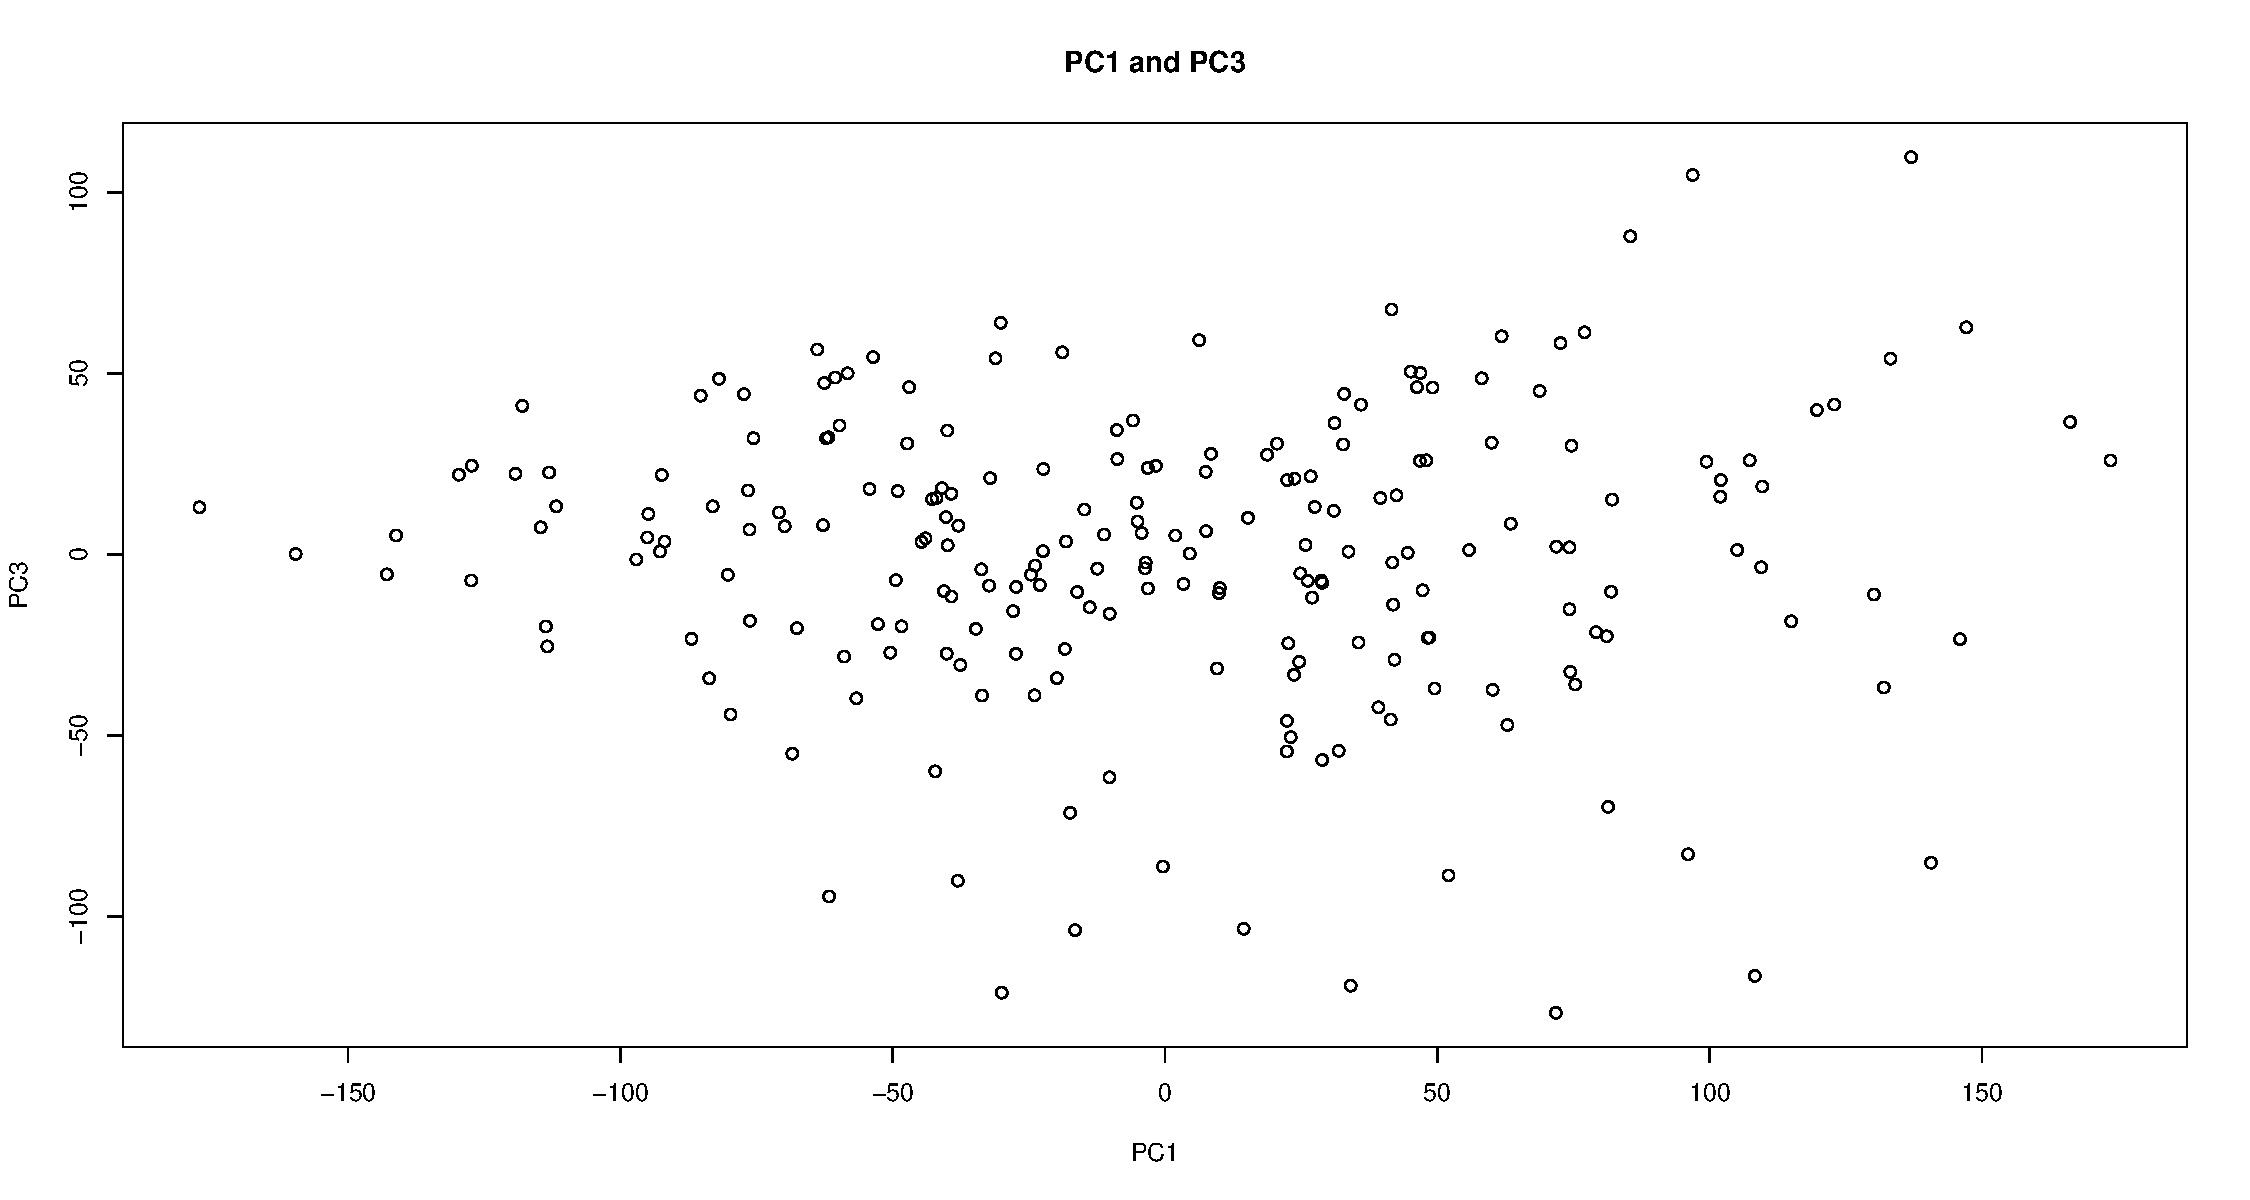
\includegraphics[width=12cm]{images/PCA (Spec)/PC1 and PC3.pdf}
    \caption{Biplot of Spectrum's PC1 and PC3}
    \label{fig:PCASpec13biplot} 
\end{figure}

\begin{figure}[H]
    \centering
    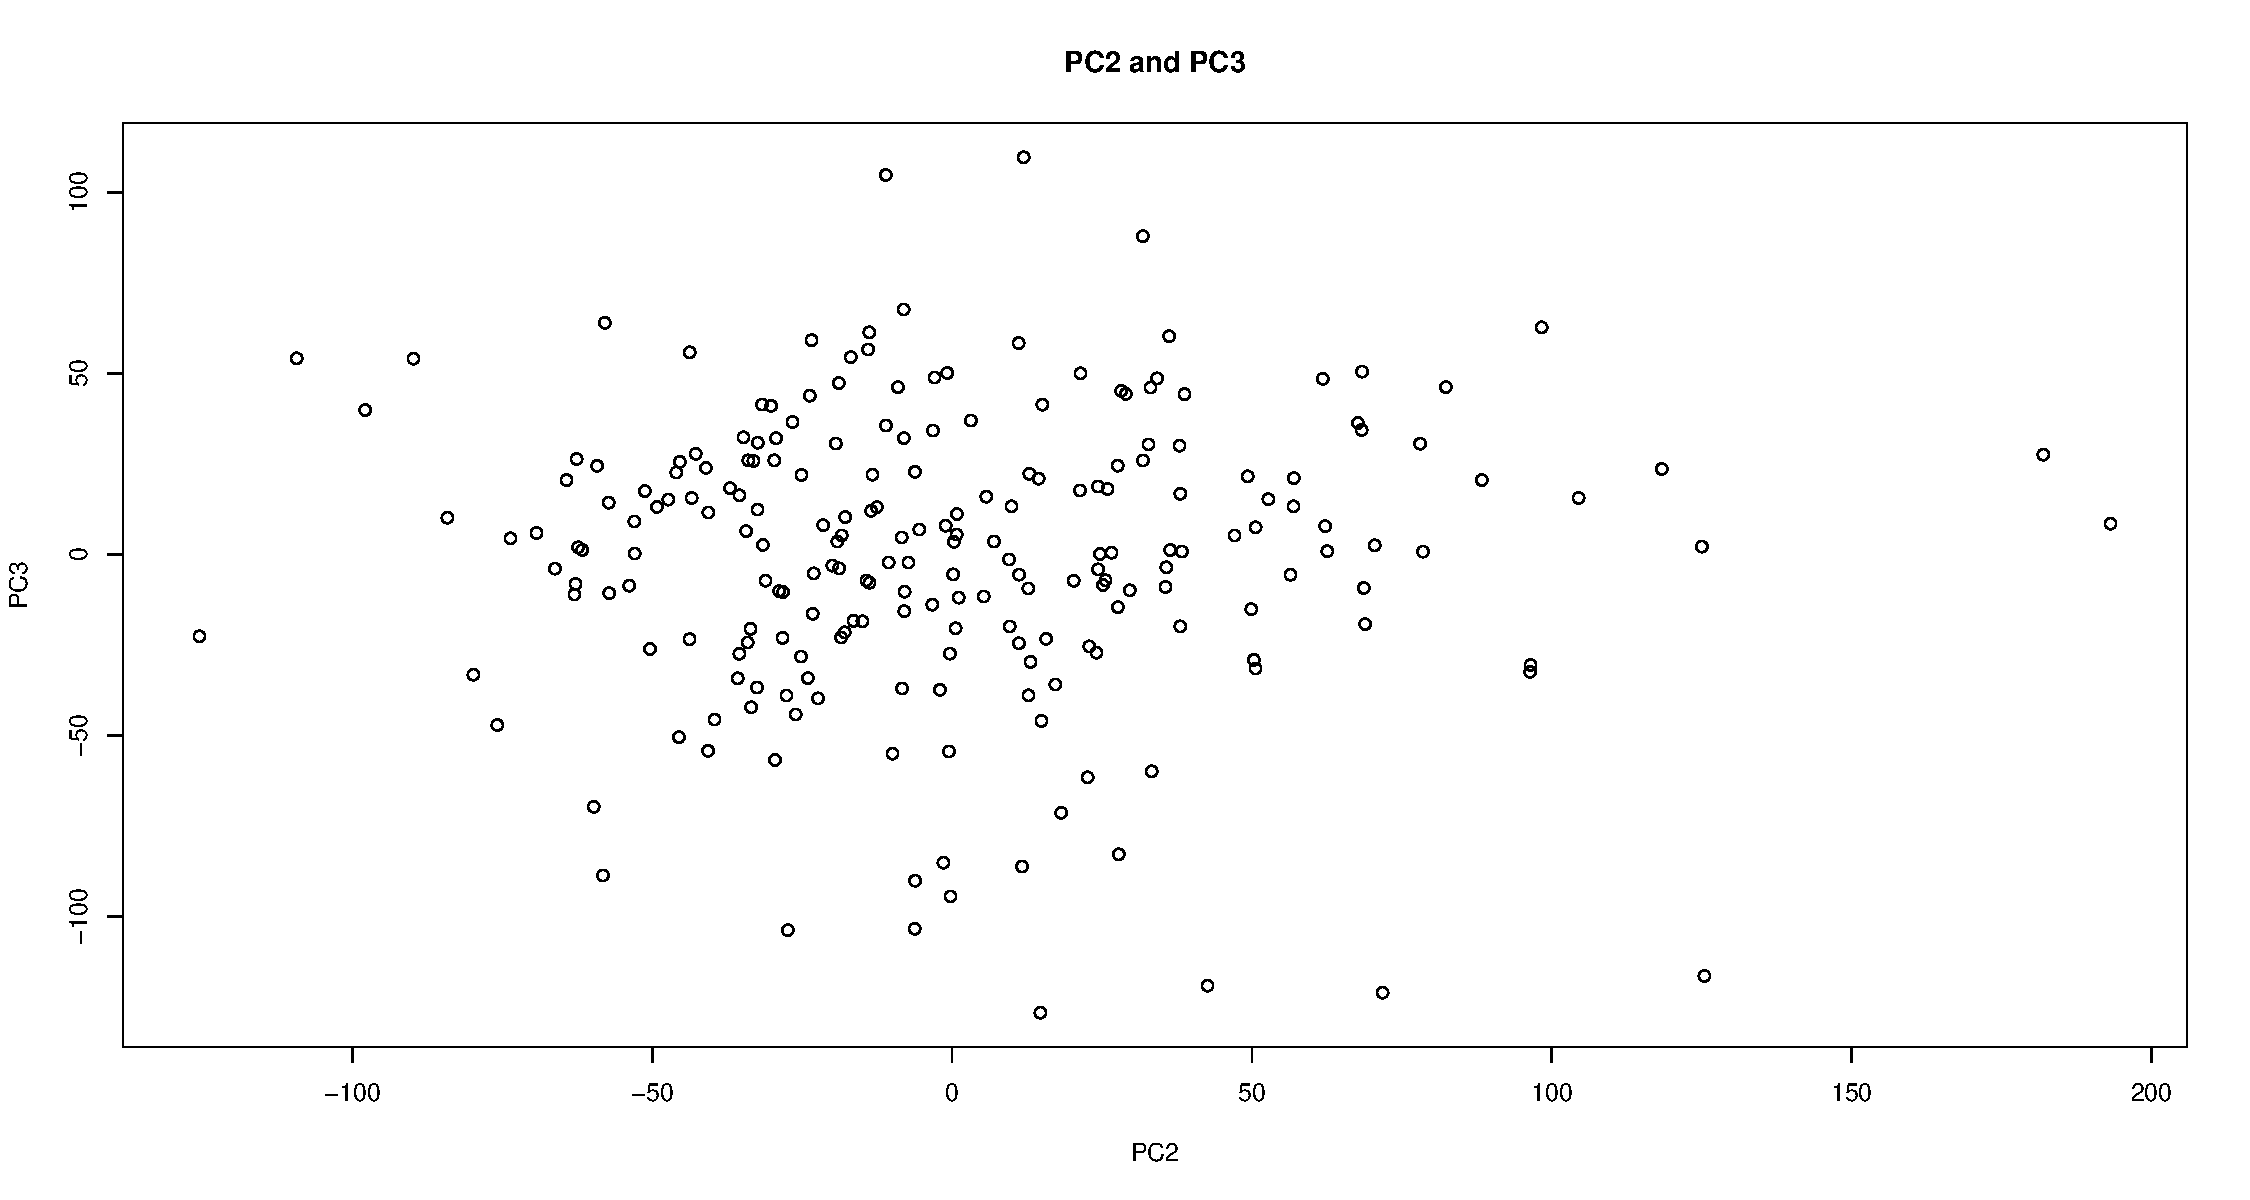
\includegraphics[width=12cm]{images/PCA (Spec)/PC2 and PC3.pdf}
    \caption{Biplot of Spectrum's PC2 and PC3}
    \label{fig:PCASpec23biplotd} 
\end{figure}

We can see that there is a much wider spread on the biplots between the three principal components compared to the case of original dataframe. There seems to be no obvious observable cluster groups among the three biplots, which can be interpreted that the three principal components are all widely spread and has moderate variance.
This may be due to the difference in the length of each spectrum, since it almost has 4 times difference from the original dataframe.

Now we should calculate and compare the variance for each 219 principal components. Then we calculate the proportion of variance of each principal components and produce a scree plot.

\begin{figure}[H]
    \centering
    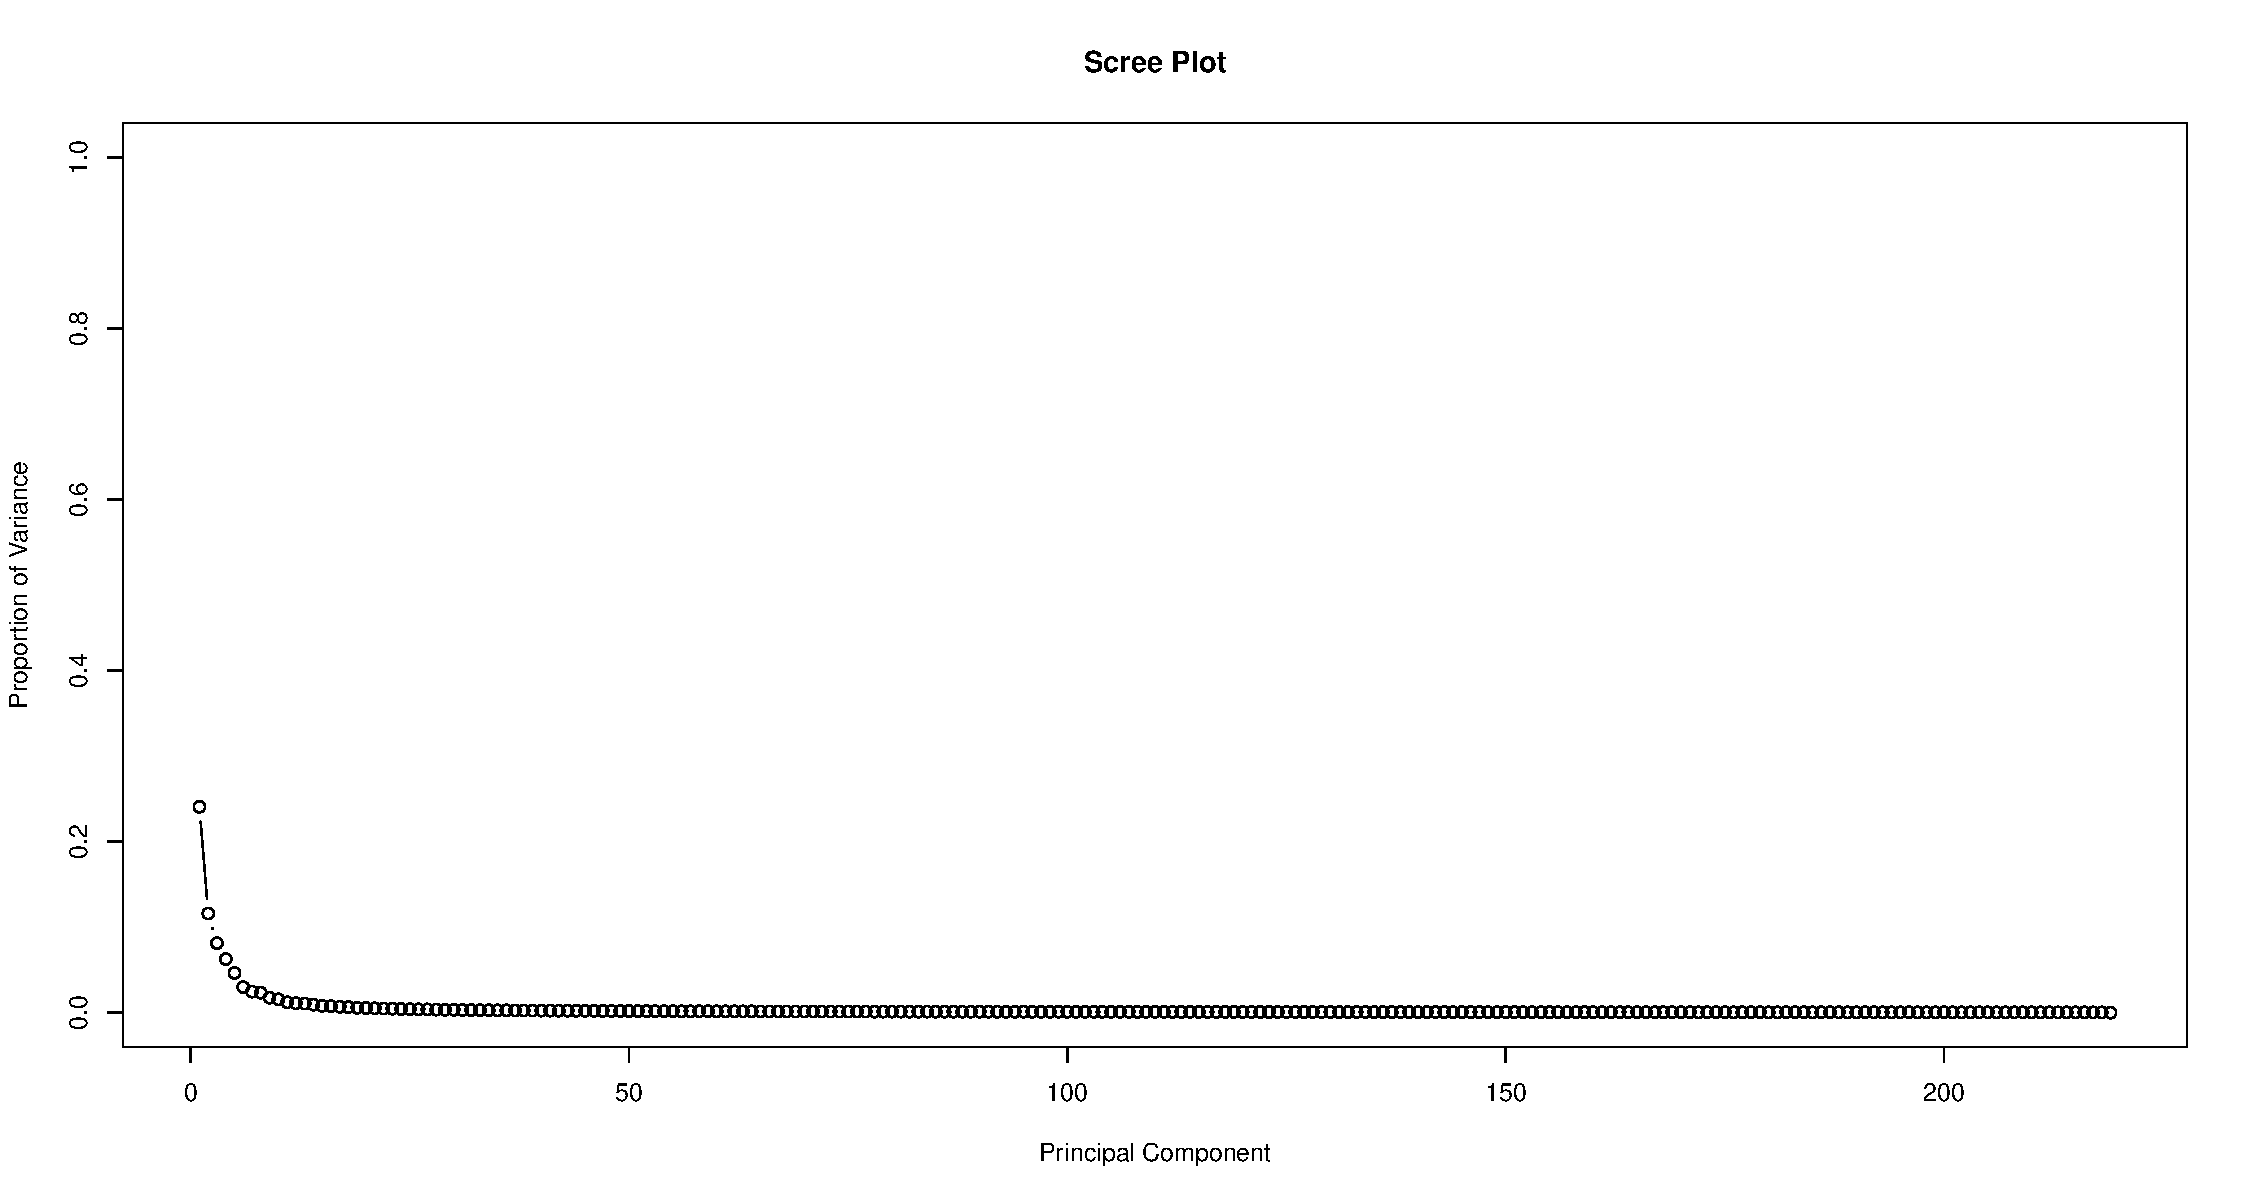
\includegraphics[width=12cm]{images/PCA (Spec)/Scree Plot.pdf}
    \caption{Spectrum's Scree Plot}
    \label{fig:Spec screeplot} 
\end{figure}

We can also construct a cumulative scree plot, which has y-axis as the cumulative proportion of variance instead.

\begin{figure}[H]
    \centering
    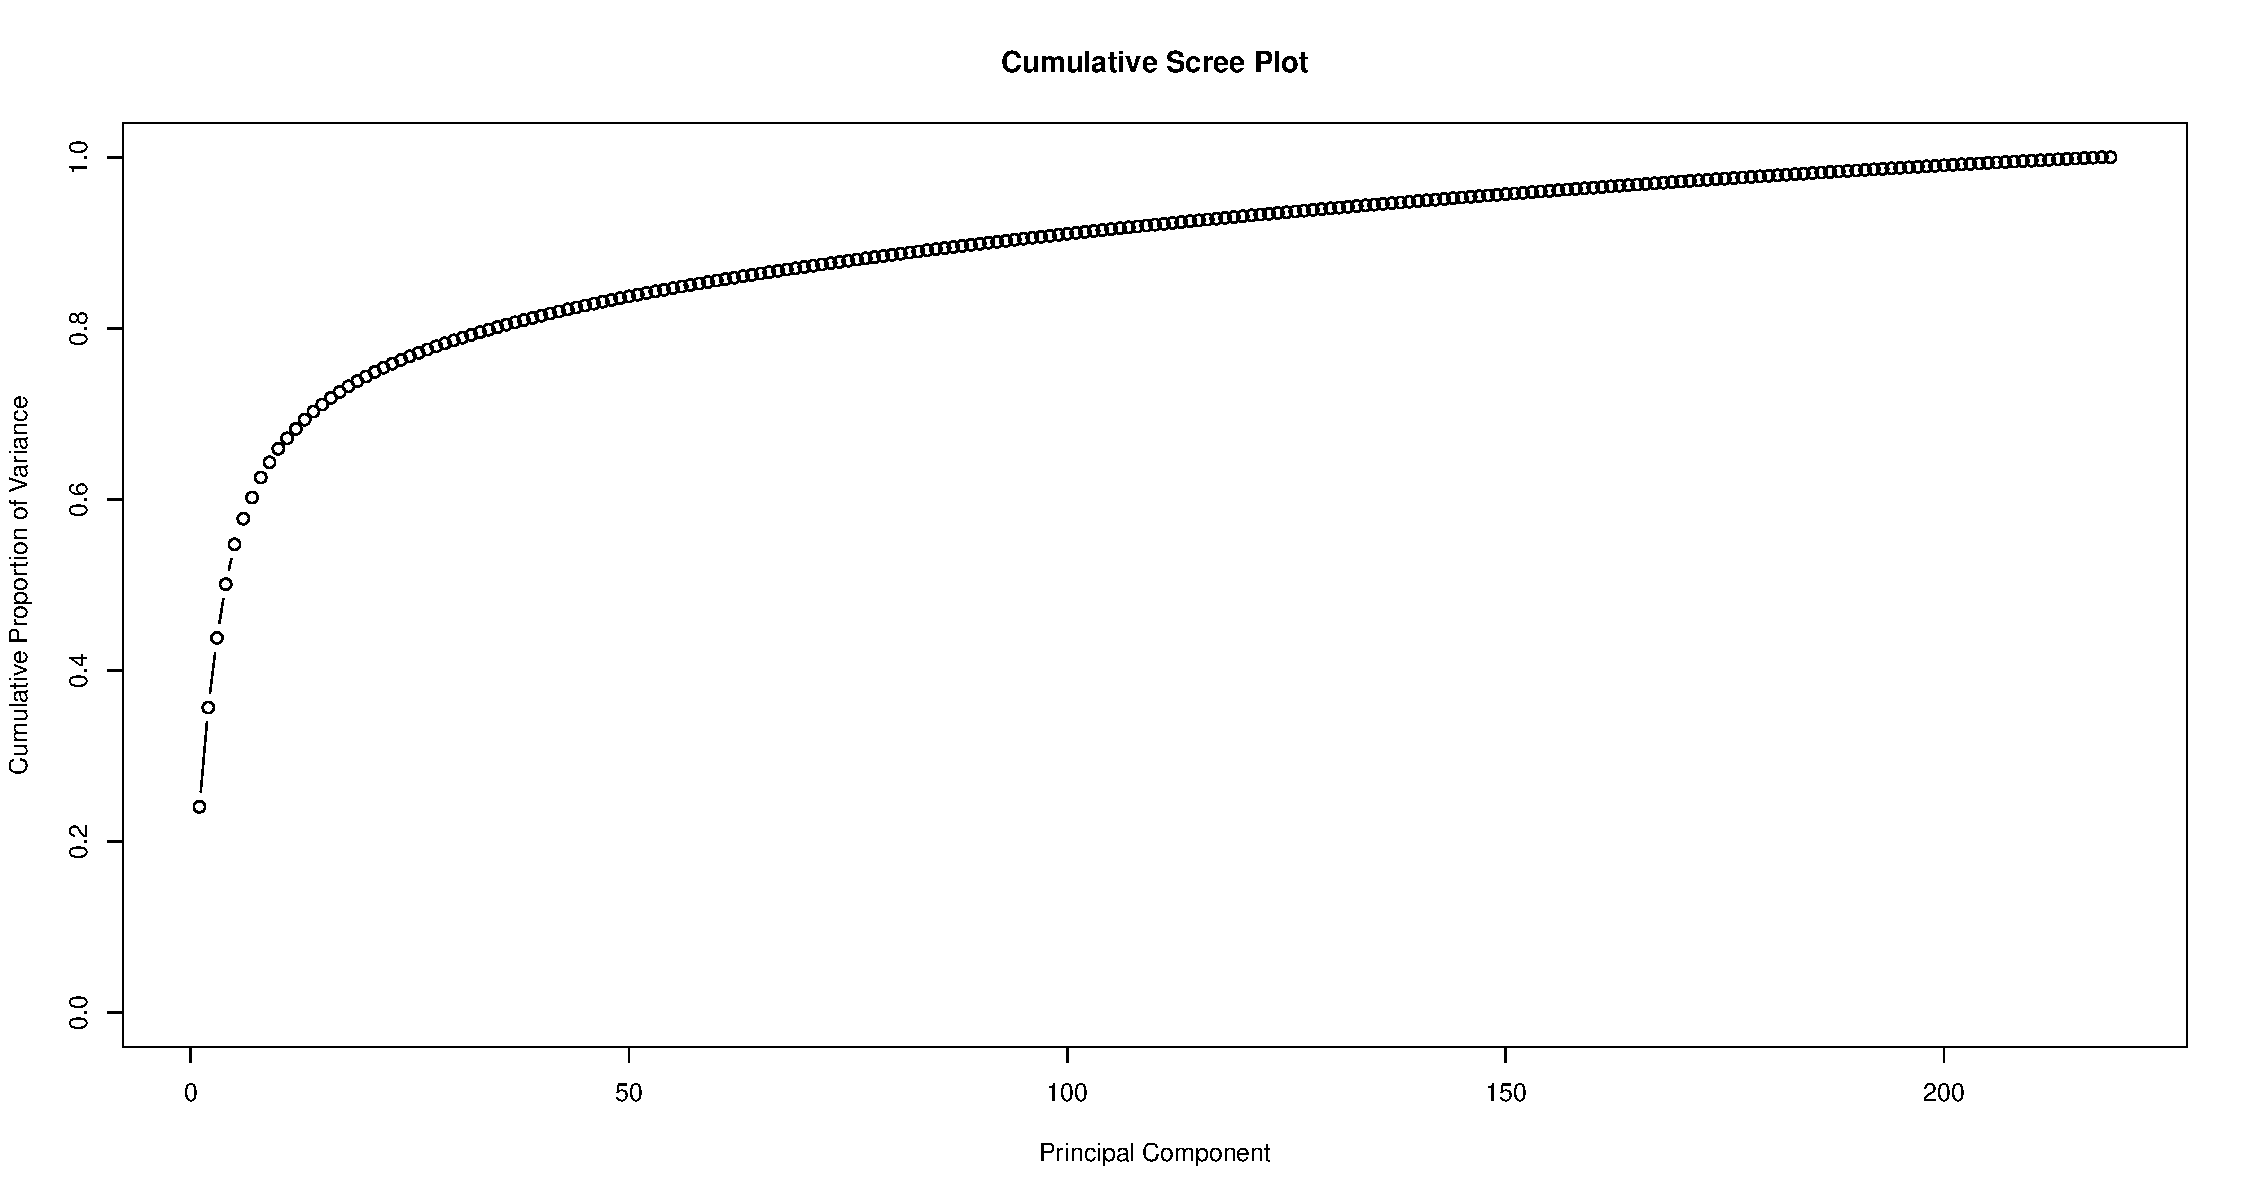
\includegraphics[width=12cm]{images/PCA (Spec)/Cumulative Scree Plot.pdf}
    \caption{Spectrum's Cumulative Scree Plot}
    \label{fig:Spec cumscreeplot} 
\end{figure}

We can notice from the plot that the first three principal components contributes to roughly 20 percent of the total variance and the first 12 principal components contributes to roughly 40 percent of the total variance.

We can notice that the first principal component contributes significantly higher in variance than the rest, up to roughly 21 percent of the total variance. Although the first principal component has a significant difference in the variance than the others, the second and third principal component also contributes to a substantial amount of variance, which supports the observations from figure 12, 13, and 14. The first three principal components contributes to roughly 42 percent of the total variance and the first 7 principal components contributes to roughly 60 percent of the total variance.

Compared to the results from original dataframe, we can observe that the first few key principal components contributes to a much more significant amount of variance in the results from spectrum dataframe.

We can now compute the number of principal components to use and to neglect, depending on the percentage of the variance. In order to take account of 80 percent of the variance we get a calculated result of 35 (roughly 84 percent reduction in dimension). In order for 90 percent and 95 percent we get a calculated result of 92 (roughly 58 percent reduction in dimension) and 142 (roughly 35 percent reduction in dimension) each. 

In conclusion the overall result of the principal component analysis applied on spectrum of 219 acoustic signal data resulted on generating 219 principal components. By calculating the proportion of variance, we concluded with a calculation that roughly 84, 58, and 35 percent of dimension out of 219 dimensions can be reduced in order to consider 80 , 90, 95 percent of variance. 

Notice that for the 80 percent of variance, PCA on spectrum dataframe has a much more efficient outcome compared to original dataframe (roughly 8.5 percent more reduction). However, PCA on original dataframe becomes much more efficient for 90, 95, and further percent of variance (roughly 6 and 17 percent more reduction).


\newpage
\subsection{PCA on original dataframe separated by language}


Now we perform the PCA on original dataframe separated by the five romance langauges: Portuguese, Italian, Iberian Spanish, French, and American Spanish. First we divide the dataframe \emph{finalDF} into parts that corresponds to each languages (Portuguese, Italian, Iberian Spanish, French, and American Spanish) and save them in objects \emph{finalDFPO, finalDFIT, finalDFSI, finalDFFR, finalDFSA}. Index 1 to 25 of \emph{finalDF} consists of Portuguese, 27 to 75 on Italian, 76 to 113 on Iberian Spanish, 114 to 173 on French, and 174 to 219 on American Spanish. The length of the index is the dimension for each languages.

Now we perform PCA on the five dataframe objects \emph{finalDFPO, finalDFIT, finalDFSI, finalDFFR, finalDFSA}. 

The following figures are the biplots for first three principal components and the cumulative scree plot for the dataframe \emph{finalDFPO}.

\begin{figure}[H]
    \centering
    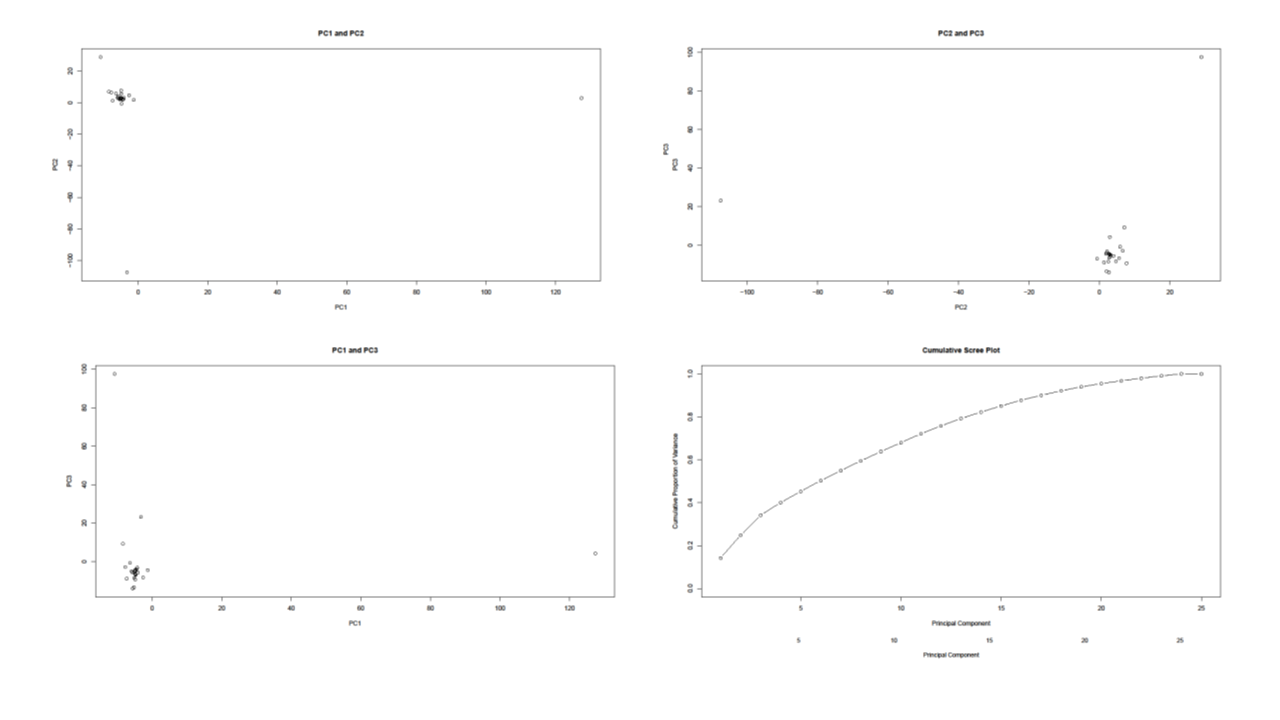
\includegraphics[width=15cm]{images/PCA/4plotPO.png}
    \caption{Biplot and Screeplot of Portuguese Dataframe}
    \label{fig:4plotPO} 
\end{figure}

We can observe that the three biplots all form a strongly gathered cluster group with negligible number of outliers.

Out of total 25 principal components, in order to take account of 80 percent of the variance we get a calculated result of 14 (roughly 44 percent reduction in dimension). In order for 90 percent and 95 percent we get a calculated result of 17 (roughly 32 percent reduction in dimension) and 20 (roughly 20 percent reduction in dimension) each. 

Notice that the three biplots of the first three principal components forms a highly gathered cluster.

The following figures are the biplots for first three principal components and the cumulative scree plot for the dataframe \emph{finalDFIT}.

\begin{figure}[H]
    \centering
    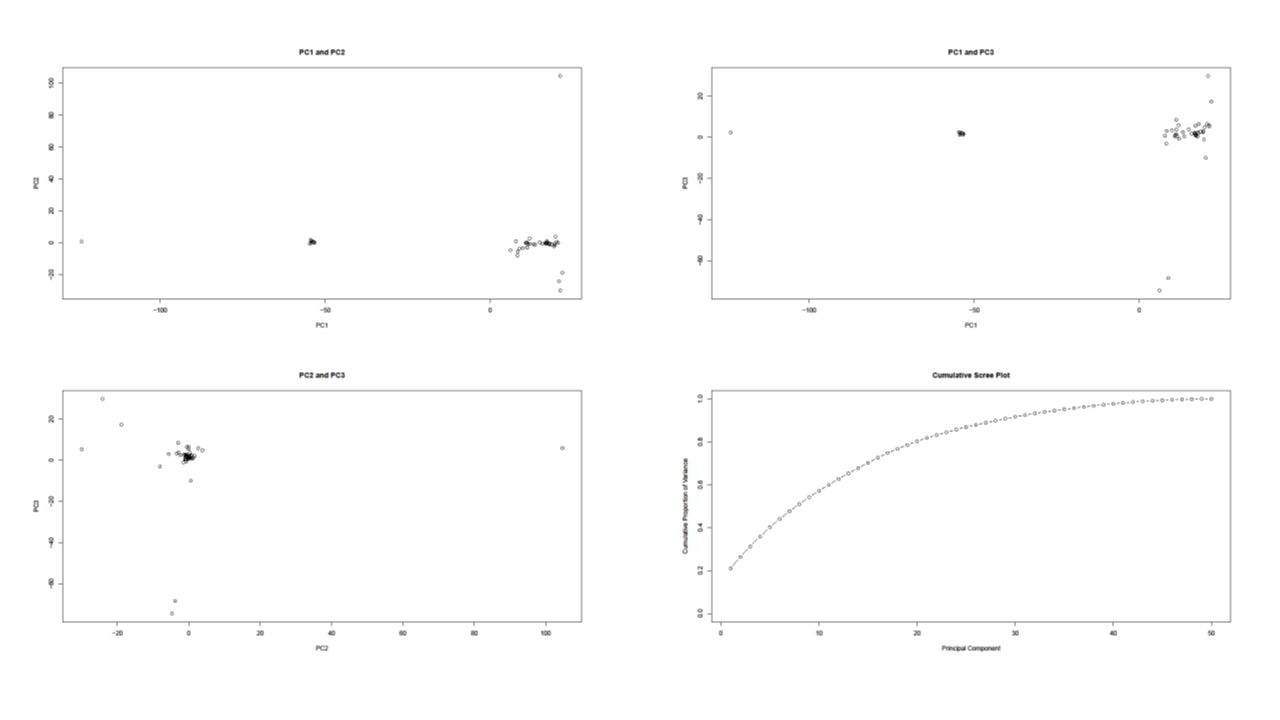
\includegraphics[width=15cm]{images/PCA/4plotIT.png}
    \caption{Biplot and Screeplot of Italian Dataframe}
    \label{fig:4plotIT} 
\end{figure}

We can observe that the three biplots all form a moderately gathered cluster group with some number of outliers, even forming a trivial cluster group on the top two figures.

Out of total 50 principal components, in order to take account of 80 percent of the variance we get a calculated result of 20 (roughly 60 percent reduction in dimension). In order for 90 percent and 95 percent we get a calculated result of 29 (roughly 42 percent reduction in dimension) and 35 (roughly 30 percent reduction in dimension) each. 

The following figures are the biplots for first three principal components and the cumulative scree plot for the dataframe \emph{finalDFSI}.

\begin{figure}[H]
    \centering
    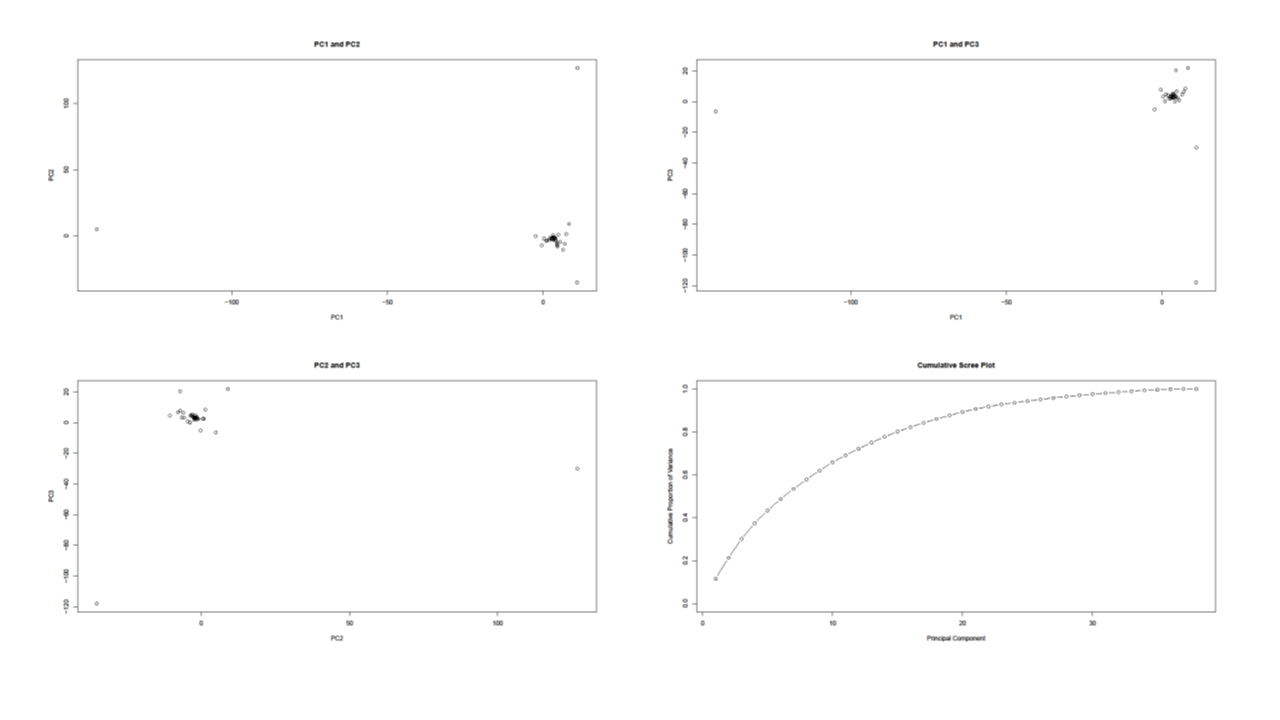
\includegraphics[width=15cm]{images/PCA/4plotSI.png}
    \caption{Biplot and Screeplot of Iberian Spanish Dataframe}
    \label{fig:4plotSI} 
\end{figure}

We can observe that the three biplots all form a strongly gathered cluster group with negligible number of outliers, similar to observation from the Portuguese dataframe.

Out of total 38 principal components, in order to take account of 80 percent of the variance we get a calculated result of 15 (roughly 60.5 percent reduction in dimension). In order for 90 percent and 95 percent we get a calculated result of 21 (roughly 45 percent reduction in dimension) and 26 (roughly 31.5 percent reduction in dimension) each. 

The following figures are the biplots for first three principal components and the cumulative scree plot for the dataframe \emph{finalDFFR}.

\begin{figure}[H]
    \centering
    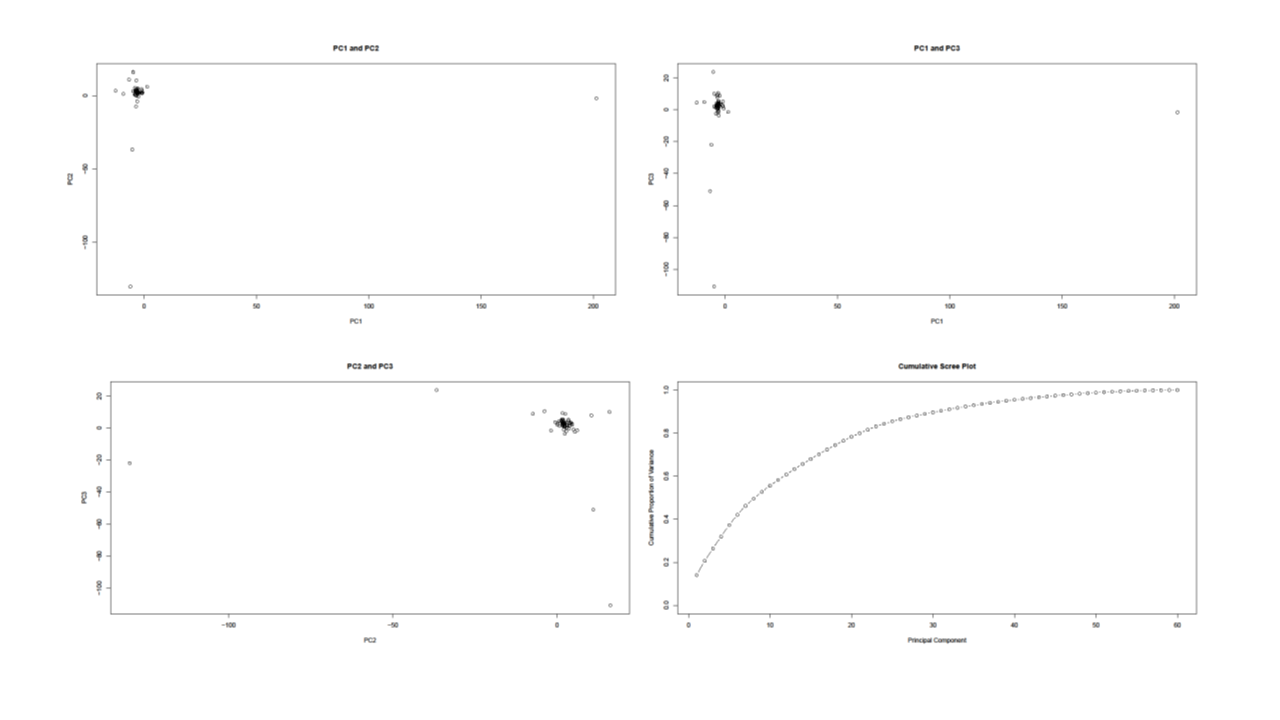
\includegraphics[width=15cm]{images/PCA/4plotFR.png}
    \caption{Biplot and Screeplot of French Dataframe}
    \label{fig:4plotFR} 
\end{figure}

We can observe that the three biplots all form a strongly gathered cluster group with few number of outliers, similar to observation from the Portuguese and Iberian Spanish dataframe.

Out of total 60 principal components, in order to take account of 80 percent of the variance we get a calculated result of 22 (roughly 63 percent reduction in dimension). In order for 90 percent and 95 percent we get a calculated result of 31 (roughly 48.5 percent reduction in dimension) and 39 (roughly 35 percent reduction in dimension) each. 

The following figures are the biplots for first three principal components and the cumulative scree plot for the dataframe \emph{finalDFSA}.

\begin{figure}[H]
    \centering
    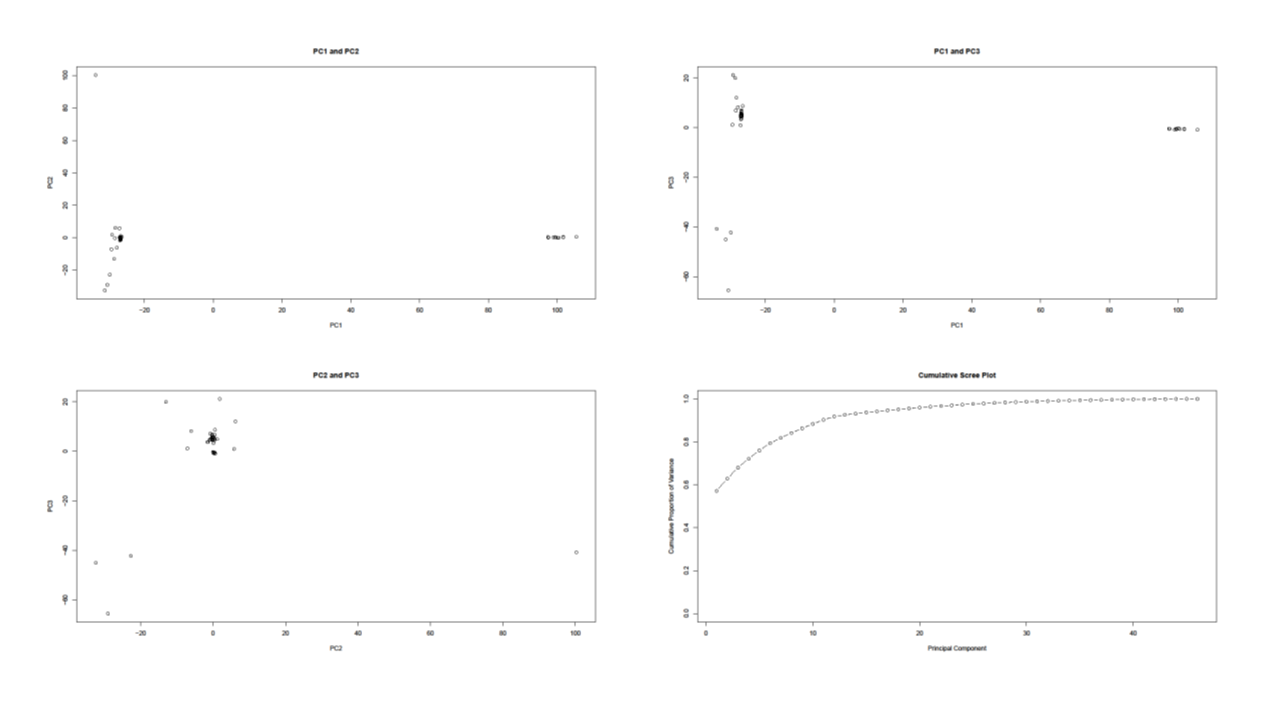
\includegraphics[width=15cm]{images/PCA/4plotSA.png}
    \caption{Biplot and Screeplot of American Spanish Dataframe}
    \label{fig:4plotSA} 
\end{figure}

We can observe that the three biplots does not form a strong and uniform cluster groups, and has the most spread and variance among the five language group dataframes.

Out of total 46 principal components, in order to take account of 80 percent of the variance we get a calculated result of 7 (roughly 85 percent reduction in dimension). In order for 90 percent and 95 percent we get a calculated result of 11 (roughly 76 percent reduction in dimension) and 18 (roughly 61 percent reduction in dimension) each. 

Notice the significantly high percent of reduction in dimension along all range of percent of variance. By observing the cumulative scatter plot, we can understand that it is due to substantially high contribution by the first principal component.